Event selection is applied that selects events compatible with containing a $\ell\tau_{\mathrm{had}}\bbbar$ final state. This selection forms the signal region containing the set of events that are used for the fit of the MVA discriminant distributions as described in Section~\ref{sec:fit}. Events must meet the following requirements
(using the object definitions described in section \ref{sec:reco}):
\begin{itemize}
\item SLT events:
	\begin{itemize}
		\item Exactly one electron passing the `tight' identification criteria, or one muon passing the `medium' identification criteria 
		%(that also includes a requirement that the muon must have | $\eta$ | < 2.5), 
		with $\pT$ 1 $\GeV$ above the corresponding trigger threshold used in that data-taking period.
		\item Exactly one hadronic $\tau$ with \pT > 20 $\GeV$ and |$\eta$| < 2.3.
		\item At least two jets in the event with \pT > 45 (20) $\GeV$ for the leading (sub-leading) jet.
	\end{itemize}
\item LTT events:
	\begin{itemize}
		\item Exactly one electron passing the `tight' identification criteria and with \pT > 18 $\GeV$, or one
 		muon passing the `medium' identification criteria with \pT > 15 GeV. 
		An upper limit on the \pT corresponding to the equivalent SLT thresholds for that data-taking period is applied.
		Electrons are required to pass the `tight' isolation working point for ETT, 
		since the single-leg electron trigger SFs are not available for loose iso electrons.  
		(Tightening the electron isolation cut leads to 4.7\% (4.1\%) lost in ggF (VBF) non-resonant signal yields in the LTT category.) 
		\item Exactly one hadronic $\tau$ with \pT > 30 $\GeV$ and |$\eta$| < 2.3.
		\item The \pT thresholds on the leading and sub-leading jets depend on the 
		corresponding trigger applied. Trigger list can be found in \ref{sec:lephadtrigger}.
		\begin{itemize}
			\item For the $e\tau$ trigger (2017-2018), since OR of two triggers are applied, the one that requires lower jet \pT threshold is prioritized.
			\item For the $\mu\tau$ trigger (2017-2018), two different jet \pT thresholds are applied for $\pT^{\tau}$ > 40 $\GeV$ and 30 < $\pT^{\tau}$ < 40 $\GeV$ since different triggers are applied for these two regions.
			\item The \pT thresholds applied are as follows:
				 \begin{itemize}
					\item If the applied trigger is seeded by L1 with J25 requirement, 
					at least two jets in the event with \pT > 80 (20) $\GeV$ for the leading (sub-leading) jet are required.
					\item If the applied trigger is seeded by L1 with 3J12 or 4J12 requirement,
					at least two jets in the event with \pT > 45 $\GeV$ are required.
					\item If there is no jet requirement at L1, at least two jets in the event with \pT > 45 (20) $\GeV$ for the leading (sub-leading) jets are required.
				\end{itemize}
		\end{itemize}
	\end{itemize}
\item No other electrons or muons in the event.
\item Opposite-sign charge between the $\tau$ and the light lepton ($e/\mu$).
\item Exactly two $b$-tagged jets (using DL1r 77\% working point).
\item The invariant mass of the \bbbar system, \mbb, is required to be < 150 GeV.
\item The invariant mass of the di-$\tau$ system (calculated using the Missing Mass Calculator (MMC) \cite{Elagin:2010aw}),
$\mMMC_{\tau\tau}$, must be > 60 $\GeV$.
\end{itemize}

\begin{figure}
\centering
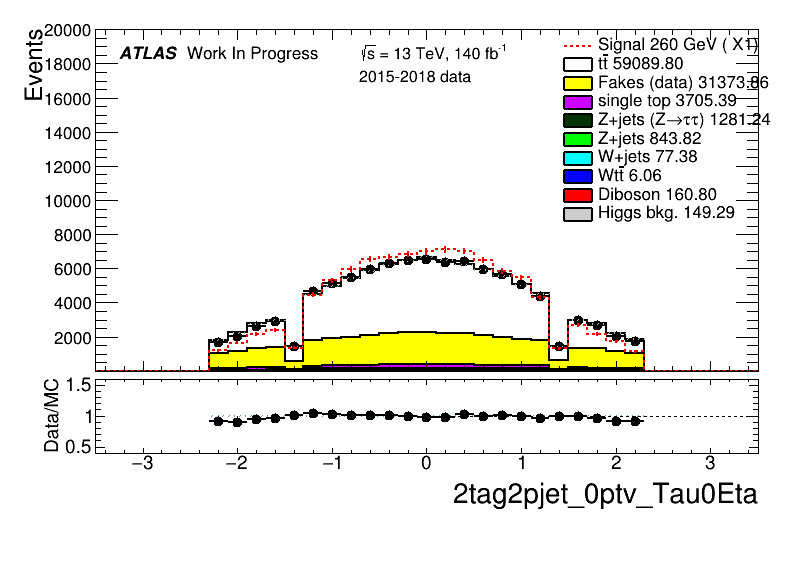
\includegraphics[width=.45\textwidth]{figures/selection/2tag2pjet_0ptv_Tau0Eta_SR_ALLFAKES_SLT_ALL_NR_TRBins.png}
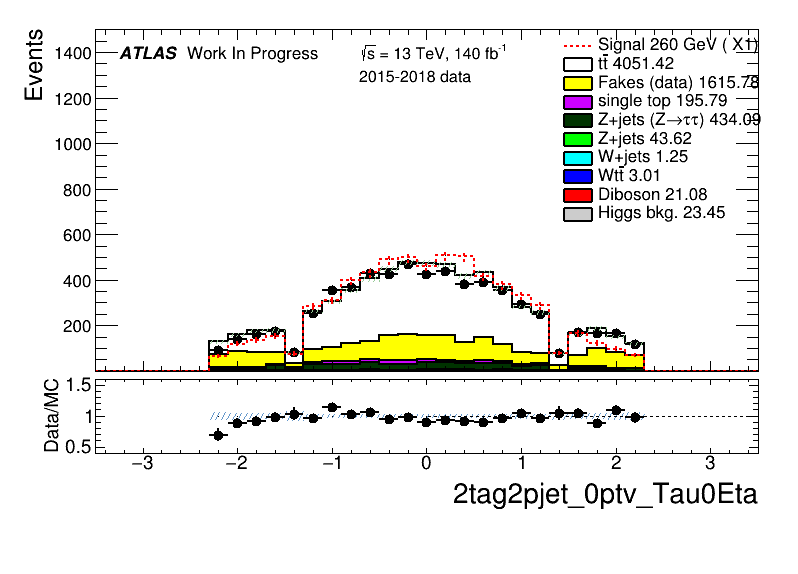
\includegraphics[width=.45\textwidth]{figures/selection/2tag2pjet_0ptv_Tau0Eta_SR_ALLFAKES_LTT_ALL_NR_TRBins.png} \\
\caption{Plots of $\tau$ $\eta$, demonstrating that the signal (scaled to the integral of the background) peaks more sharply at zero than the background in the \lephad channel. Included for the (left) single lepton trigger channel and (right) lepton-plus-tau trigger channel.}
\label{fig:tau_eta_23}
\end{figure}

The selection for $\tau$ $|\eta|$ to be less than 2.3 differs from the selection in the hadhad channel, and has been chosen as an analysis optimization choice from previous rounds of the analysis.  As you can see in Fig.~\ref{fig:tau_eta_23}, the signal is expected to peak more sharply at low |$\eta$| than the background, so the cut at 2.3 is expected to provide a modest background reduction.

	
  
\begin{table}
    \centering
    \scriptsize
    \begin{tabular}{|c|c|c|c|c|}
    	\hline
	\hline
	SampleName & Entries & Integral & Error & Error/Integ.\\

	\hline
 	\hline    
 	hhttbbggFSM     &151522 &5.86759 & 0.0179841&0.31\% \\ 
	hhttbbVBFSM	   	&36457  & 0.20024&0.0012615&0.63\% \\
	Hhhbbtautau251	& 22541 &	60.5803  & 0.416596	& 0.69\% \\
	Hhhbbtautau260	& 22252 &	60.8690  & 0.422004	& 0.69\% \\
	Hhhbbtautau280	& 24595 &	67.9352  & 0.447715	& 0.66\% \\
	Hhhbbtautau300	& 18398 &	77.1913  & 0.588118	& 0.76\% \\
	Hhhbbtautau325	& 20904 &	90.9350  & 0.649871	& 0.71\% \\
	Hhhbbtautau350	& 23593 &	106.391  & 0.716122	& 0.67\% \\
	Hhhbbtautau400	& 29280 &	140.007  & 0.845998	& 0.60\% \\
	Hhhbbtautau450	& 34665 &	175.289  & 0.973111	& 0.56\% \\
	Hhhbbtautau500	& 21332 &	210.657  & 1.48889	& 0.71\% \\
	Hhhbbtautau550	& 23571 &	240.878  & 1.62159	& 0.67\% \\
	Hhhbbtautau600	& 25917 &	273.858  & 1.75829	& 0.64\% \\
	Hhhbbtautau700	& 29596 &	327.036  & 1.96578	& 0.60\% \\
	Hhhbbtautau800	& 32606 &	374.464  & 2.14260	& 0.57\% \\
	Hhhbbtautau900	& 34392 &	405.559  & 2.26269	& 0.56\% \\
	Hhhbbtautau1000	& 35119 &	425.155  & 2.34509	& 0.55\% \\
	Hhhbbtautau1100	& 44157 &	416.216  & 2.04469	& 0.49\% \\
	Hhhbbtautau1200	& 32337 &	386.871  & 2.43156	& 0.63\% \\
	Hhhbbtautau1400	& 25539 &	251.079  & 1.62164	& 0.65\% \\
	Hhhbbtautau1600	& 14421 &	160.598  & 1.39334	& 0.87\% \\
	\hline
	
	Fake     	  &	2054613  & 35834.2   & 116.072    &	0.32\% \\
	ttbar     	  &	490058    & 61707.2   & 91.4456    & 0.15\% \\
	stopWt 	   &	25910      & 3068.72   & 19.8006    & 0.65\% \\
	stopt   	   &	5798        & 597.841   & 11.146      &	1.86\% \\
	stops 	   &	1450        & 38.0965   & 1.0672      &	 2.80\% \\
	Zbb 		   &	17645      & 577.445   & 18.6845    &	 3.24\% \\
	Zbc 		   &	1467        & 57.1754   & 7.31240    &	 12.79\% \\
	Zbl 	            &	1006        & 39.4660   & 5.89920    &	 14.95\% \\
	Zcc 	            &	278 	        & 63.3618   & 16.3586    &	 25.82\% \\
	Zcl	            &	135          & 23.1748   & 10.38491   & 44.81\% \\
	Zl	            &	30            & 5.1560     & 2.5307       & 49.08\% \\
	Zttbb 	    &	21473      & 1034.74   & 19.7203     & 1.91\% \\
	Zttbc 	    &	1746        & 100.9634 & 7.84392     & 7.77\% \\
	Zttbl 		    &	1184        & 62.7492   & 6.58925     & 10.50\% \\
	Zttcc 	    &	608          & 118.2826 & 21.84047   & 18.46\% \\
	Zttcl		    &	216          & 12.6376   & 9.48049     & 75.02\% \\
	Zttl 		    &	122          & 15.5227   & 5.58566     & 35.98\% \\
	W 		    &	747          & 77.4938   & 8.40607     & 10.85\% \\
	DY                &	68            & 13.5159   & 3.40597     & 25.20\% \\
	Wtt               &	76            & 5.51685   & 0.816626   & 14.80\% \\
	DYtt              &	9              & 2.6588     & 1.72628     & 64.93\% \\
	WW              &	110          & 14.0836   & 2.19759     & 15.60\% \\
	WZ               &	1992        & 60.1072   & 2.73295     & 4.55\% \\
	ZZ 		    &	6754        & 84.6051   & 2.08094     & 2.46\% \\
	VBFHtautau &	933          & 1.4224     & 0.0491357 & 3.45\% \\
	ggFHtautau  &	2159        & 17.1723   & 0.443422   & 2.58\% \\
	ggZHtautau  &	838          & 2.87863   & 0.10284     & 3.57\% \\
	ZHtautau      &	1923        & 8.497219 & 0.206055   & 2.42\% \\
	WHtautau     &	92            & 0.714224 & 0.0805373 & 11.28\% \\
	ZHbb            &	88889      & 23.4744   & 0.252781   & 1.08\% \\
	WHbb           &	6054        & 6.94652   & 0.143376   & 2.06\% \\
	ttH                &	37692      & 58.0919   & 0.312495   & 0.54\% \\
	\hline
	
 	\hline
	total bkg  & 2772080 & 103734.0 & &\\
	data         & 98456     & 98456	& &\\
 	\hline
 	\hline
	  
      \end{tabular}
      \caption{Pre-fit event yields in the di-Higgs $bb\lephad$ SLT signal region for the data, background and signal. Here, Zttjj represents the processes as $Z\rightarrow\tau\tau + jj$,
      whereas Zjj represents  $Z\rightarrow ee/\mu\mu + jj$.}
      \label{tab:LepHadSLTYields}
\end{table}
  

\begin{table}
    \centering
    \scriptsize
    \begin{tabular}{|c|c|c|c|c|}
	
	\hline
	\hline
	SampleName & Entries & Integral & Error & Error/Integ.\\
	
	\hline
	\hline
	hhttbbggFSM    &35045	 &1.416186  &	0.008843 & 0.62\%\\	
	hhttbbVBFSM	   &10188  	&0.054756 	&0.00063987&1.17\% \\
  	Hhhbbtautau251 & 6815	 & 17.9678  & 0.224815 & 1.25\% \\
  	Hhhbbtautau260 & 6930	 & 18.4965  & 0.22967   & 1.24\% \\
	Hhhbbtautau280 & 8145	 & 22.2273  & 0.25376   & 1.14\% \\
	Hhhbbtautau300 & 6319 	& 26.4815  & 0.34358   & 	1.30\% \\
 	Hhhbbtautau325 & 7085 	& 30.8642  & 0.37816   & 	1.23\% \\
  	Hhhbbtautau350 & 7896 	& 35.9407  & 0.41597   & 	1.16\% \\
  	Hhhbbtautau400 & 8780 	& 42.5375  & 0.46722   & 	1.10\% \\
        Hhhbbtautau450  & 9303 	& 47.4140  & 0.50589  &  	1.07\% \\
	Hhhbbtautau500  & 5177 	& 51.6729  & 0.73896  & 	1.43\% \\
	Hhhbbtautau550  & 5123 	& 53.3731  & 0.76570  & 	1.43\% \\
	Hhhbbtautau600   & 5026 	& 53.8328 & 0.78163  & 	1.45\% \\
	Hhhbbtautau700   &	4699	 & 52.8369 & 0.79526 & 	1.51\% \\
	Hhhbbtautau800   &	4534	 & 52.7574 & 0.80652 & 	1.53\% \\
	Hhhbbtautau900   &	4285	 & 51.5907 & 0.81138 & 	1.57\% \\
	Hhhbbtautau1000 &	3820	 & 47.4054 & 0.78933 & 	1.67\% \\
	Hhhbbtautau1100 &	4436	 & 42.8090 & 0.66043 & 	1.54\% \\
 	Hhhbbtautau1200 &	2878	 & 33.9867 & 0.71017 & 	2.09\% \\	
	Hhhbbtautau1400 &	2264	 & 22.6836 & 0.49023 & 	2.16\% \\
 	Hhhbbtautau1600 &	1412	 & 16.0911 & 0.44594 & 	2.77\% \\
  	\hline
  
  	Fake 	&  39074	&	2146.46	&	41.7068  &	1.94\% \\
	ttbar           & 32873 &	4213.13     &	24.0372  &	0.57\% \\
	stopWt       & 1408   &	169.8852   &	4.70386  &	2.77\% \\
	stopt          & 246     &	26.1433     &	2.43237  &	9.30\% \\
	stops          & 61      &	1.6708       &	0.22960  &	13.74\% \\
	Zbb            & 1230   &	33.5952     &	3.98824  &	11.87\% \\
	Zbc            & 92       &	3.7974       &	0.82655  &	21.77\% \\
	Zbl             & 58       &	1.2151       &	0.88899  &	73.16\% \\
	Zcc            & 14       &	4.08084     &	3.10603  &	76.11\% \\
	Zcl             & 5         &	0.8519       &	0.60706  &	71.26\% \\
	Zl               & 2         &	0.0510206 &	0.03608  &	70.71\% \\
	Zttbb          & 7271   &	352.1282   &	10.66373&	3.03\% \\
	Zttbc           & 634    &	34.7063     &	4.07317  &	11.74\% \\
	Zttbl            & 406    &	27.8580     &	3.23106  &	11.60\% \\	
	Zttcc           & 174    &	28.1896     &	7.23583  &	25.67\% \\	
	Zttcl            & 86      &	8.4072       &	4.96063  &	59.00\% \\
	Zttl              & 57      &	10.8339     &	7.33489  &	67.70\% \\
	W                & 16      &	1.3289       &	0.34673  &	26.09\% \\	
	DY              & 6         &	0.5694       &	0.28426  &	49.93\% \\
	Wtt              & 22      &	2.69751     &	0.96584  &	35.81\% \\
	DYtt             & 3        &	0.2597       &	0.16896  &	65.06\% \\
	WW             & 4        &	0.4316       &	0.23477  &	54.40\% \\
	WZ               & 119   &	3.56164     &	0.53030  &	14.89\% \\
	ZZ                & 1360 &	17.2611     &	0.94440  &	5.47\% \\
	VBFHtautau & 235   &	0.3715       &	0.02506  &	6.74\% \\	
	ggFHtautau  & 461   &	4.5775       &	0.24447  &	5.34\% \\
	ggZHtautau  & 218   &	0.7408       &	0.05219  &	7.05\% \\
	ZHtautau      & 458   &	2.1790       &	0.10592  &	4.86\% \\
	WHtautau     & 23     &	0.1783       &	0.03965  &	22.23\% \\
 	ZHbb            & 16172&	5.3097       &	0.14934 &	 	2.81\% \\
	WHbb           & 82     &	0.1735       &	0.02609 &		15.04\% \\
	ttH                 & 5121 &	8.1182       &	0.11766 &		1.45\% \\
	\hline

        \hline
	total bkg 	&	107991  &	   7110.77 &  & \\		
	data		& 	6351      &    6351 	&  &   \\
	\hline
	\hline

    \end{tabular}
    \caption{Pre-fit event yields in the di-Higgs $bb\lephad$ LTT signal region for signal, data and background. Here, Zttjj represents the processes as $Z\rightarrow\tau\tau + jj$, 
    whereas Zjj represents  $Z\rightarrow ee/\mu\mu + jj$.}
    \label{tab:LepHadLTTYields}
\end{table}

The event yields after applying the $bb\lephad$ SLT and LTT event selections are shown in Table \ref{tab:LepHadSLTYields} and \ref{tab:LepHadLTTYields} for signal, data and background. 

Figures~\ref{fig:LepHadAccEffSLT} and \ref{fig:LepHadAccEffLTT} show the acceptance times efficiency of the \lephad SLT and LTT channel selections, respectively, for the di-Higgs resonant signals as a function of the resonance mass. \begin{figure}
\centering
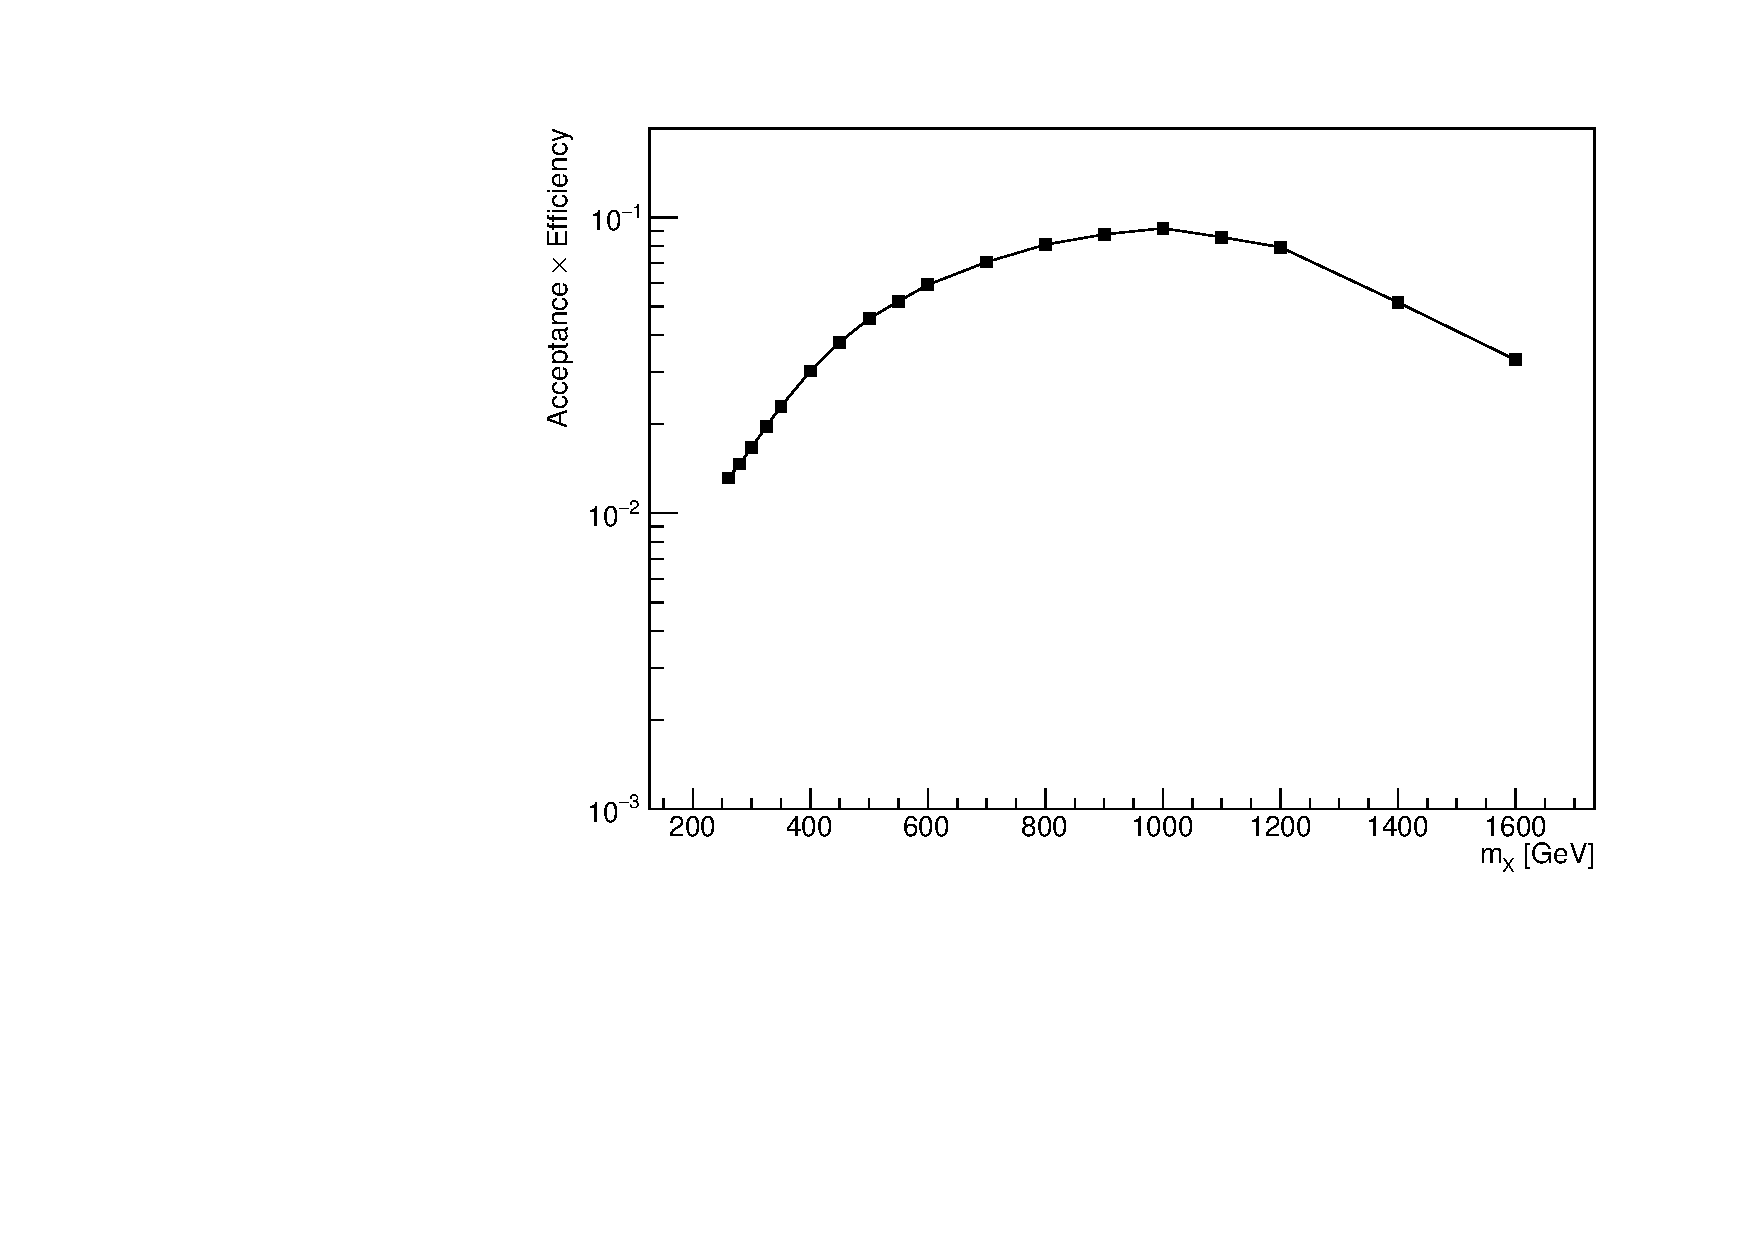
\includegraphics[width=.65\textwidth]{figures/selection/LepHad_HH/SLT_AccEff.pdf}
\caption{Acceptance times efficiency of the \lephad SLT channel selection for the di-Higgs resonant signals as a function of the resonance mass.}
\label{fig:LepHadAccEffSLT}
\end{figure}

\begin{figure}
\centering
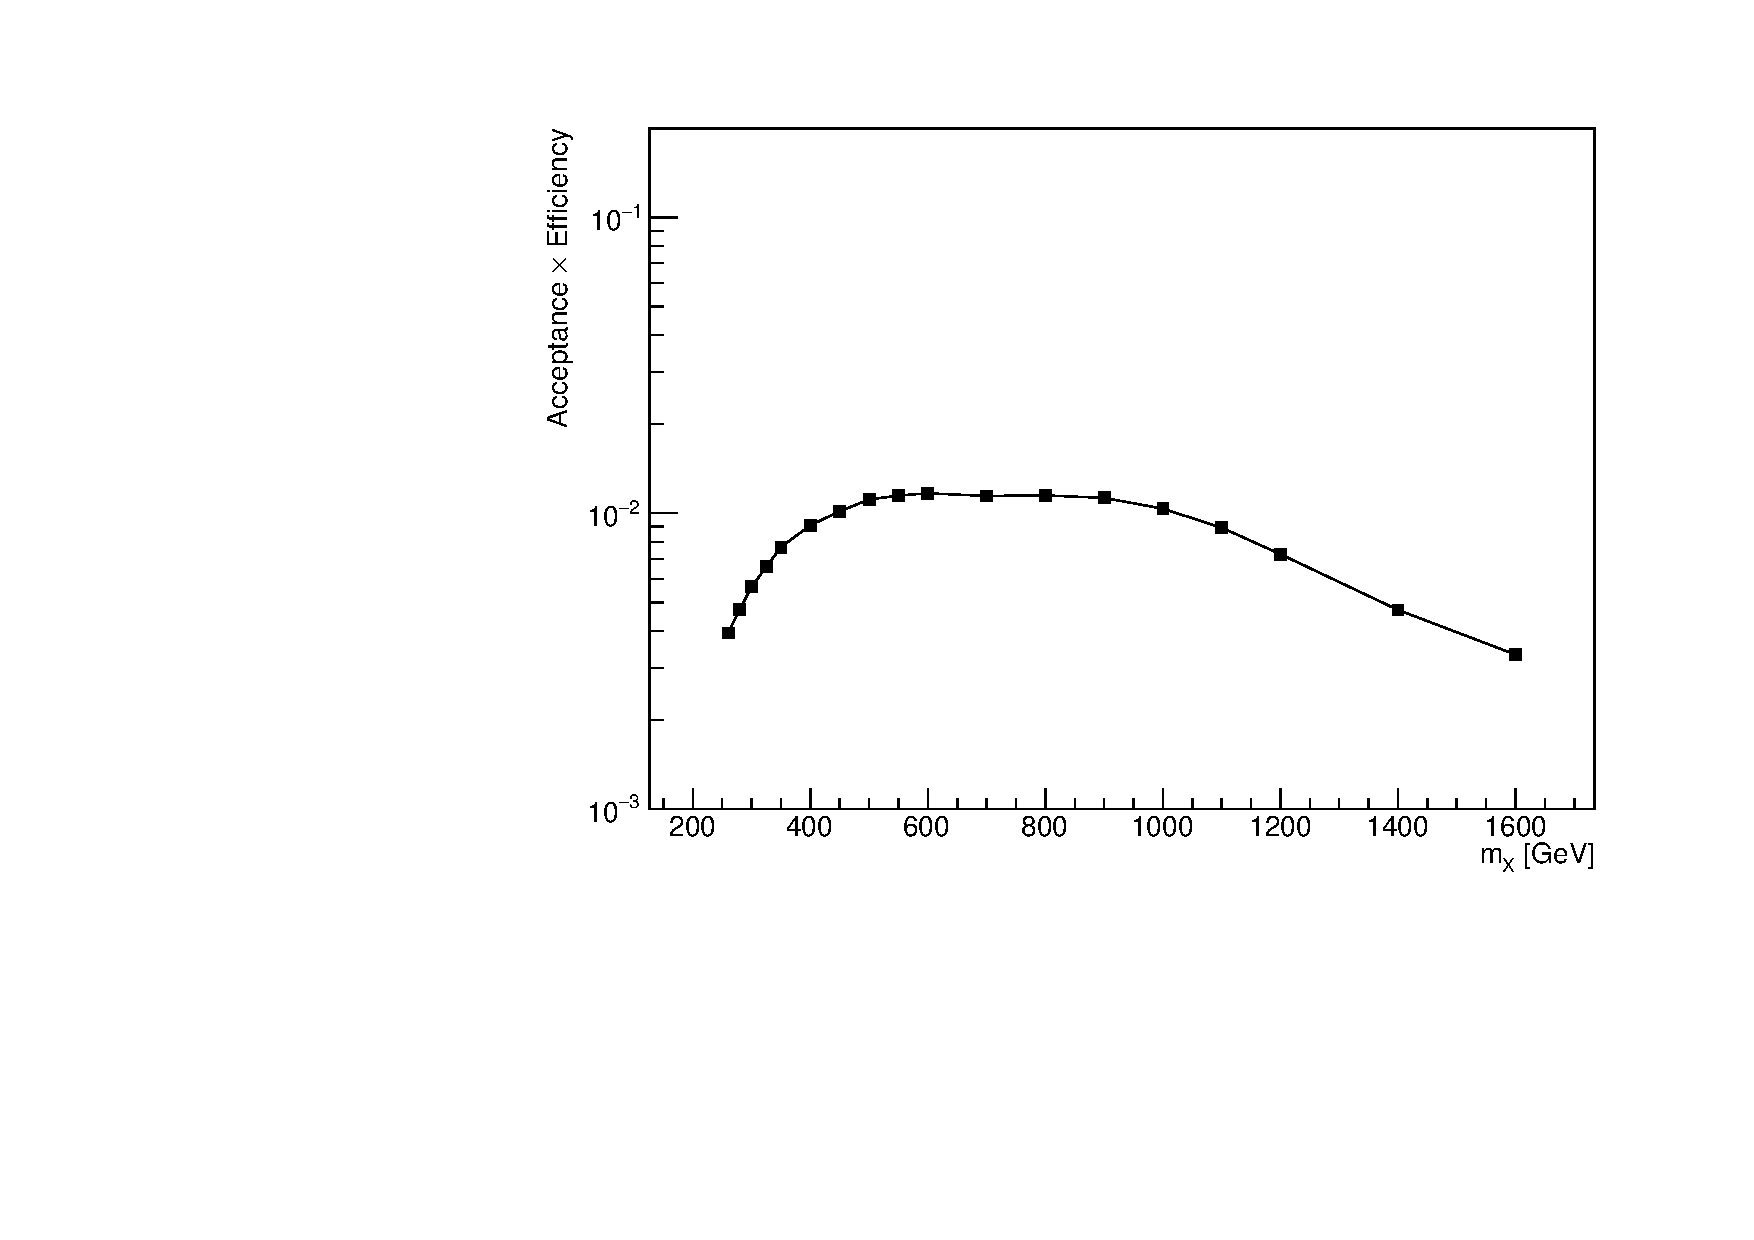
\includegraphics[width=.65\textwidth]{figures/selection/LepHad_HH/LTT_AccEff.pdf}
\caption{Acceptance times efficiency of the \lephad LTT channel selection for the di-Higgs resonant signals as a function of the resonance mass.}
\label{fig:LepHadAccEffLTT}
\end{figure}

\begin{landscape}
\begin{table}
\centering

\begin{tabular}{|c|cc|cc|cc|}
\hline
Description & \multicolumn{2}{c|}{Number of events} & \multicolumn{2}{c|}{Efficiency [\%]} & \multicolumn{2}{c|}{Relative Efficiency [\%] }\\
\hline
& SLT & LTT & SLT &  LTT &  SLT &  LTT \\
\hline
$HH$ & \multicolumn{2}{c|}{4313.87} & \multicolumn{2}{c|}{x} & \multicolumn{2}{c|}{x} \\
$HH\rightarrow bb\tau\tau$ & \multicolumn{2}{c|}{315.23} & \multicolumn{2}{c|}{x} & \multicolumn{2}{c|}{x} \\
$HH\rightarrow bb\tau_{lep}\tau_{h}$ & \multicolumn{2}{c|}{143.82} & \multicolumn{2}{c|}{100.00} & \multicolumn{2}{c|}{100.00} \\
Generator filter & \multicolumn{2}{c|}{91.98} &  \multicolumn{2}{c|}{63.96} &  \multicolumn{2}{c|}{63.96} \\
Derivation skimming & \multicolumn{2}{c|}{71.94} & \multicolumn{2}{c|}{50.02} & \multicolumn{2}{c|}{78.21} \\
Object preselection & \multicolumn{2}{c|}{27.53} & \multicolumn{2}{c|}{19.14} & \multicolumn{2}{c|}{38.26} \\
\hline
Trigger selection (online+offline) & \multicolumn{2}{c|}{21.68} & \multicolumn{2}{c|}{15.08} & \multicolumn{2}{c|}{100.00} \\ 
Trigger category & 16.79 & 4.90 & 11.67 & 3.40 & 77.42 & 22.58 \\
\hline
Random tau selection & 16.79 & 4.90 & 11.67 & 3.40 & 100.00 & 100.00 \\
Object selection ($n_\tau=2$, further requirements on jets and tau-jet OLR) & 15.43 & 4.48 & 10.73 & 3.11 & 91.93 & 91.51 \\
Lepton, $\tau$,trigger eff weight &14.25&	4.26&	9.91	&2.96	&92.34&	95.01\\
$\tau$ $\eta$ Cut & 14.01 & 4.16 & 9.74 & 2.90 & 98.35 & 98.55 \\
Trigger Specific \pT cut & 13.66	&3.30	&9.50	&2.29	&97.50	&79.24 \\
Opposite charge sign & 13.48 & 3.27	&9.37&	2.28&	98.62&	99.21\\
\hline
Both jets are $b$-tagged & 6.28 & 1.52	&4.36&	1.06&	46.58&	46.35 \\
MMC > 60 GeV & 6.18 & 1.50	&4.30&	1.04&	98.52&	98.62 \\
$m_{bb} < 150$ GeV & 5.87 & 1.42	&4.08&	0.98&	94.87	&94.63 \\
\hline
\end{tabular}
\caption{Non-resonant \lephad SM ggF signal cutflow (Powheg+Pythia8).}
\label{tab:SMHH_lephad_cutflow}
\end{table}
\end{landscape}

\begin{landscape}
    \begin{table}
    \centering
\begin{tabular}{|c|cc|cc|cc|}
 \hline
 Description & \multicolumn{2}{c|}{Number of events} & \multicolumn{2}{c|}{Efficiency [\%]} & \multicolumn{2}{c|}{Relative Efficiency [\%] }\\
 \hline
 & SLT & LTT & SLT &  LTT &  SLT &  LTT \\
 \hline
 $HH$ & \multicolumn{2}{c|}{239.798} &	\multicolumn{2}{c|}{x}   & \multicolumn{2}{c|}{x}  \\
 $HH\rightarrow bb\tau\tau$ & \multicolumn{2}{c|}{17.523}  &  \multicolumn{2}{c|}{x}   & \multicolumn{2}{c|}{x} \\
 $HH\rightarrow bb\tau_{lep\tau_{h}}$ & \multicolumn{2}{c|}{7.995}   &  \multicolumn{2}{c|}{100.00} &   \multicolumn{2}{c|}{x} \\
 Generator filter & \multicolumn{2}{c|}{4.587}   &  \multicolumn{2}{c|}{57.38} &    \multicolumn{2}{c|}{57.38} 	 \\
 Derivation skimming & \multicolumn{2}{c|}{3.429}   &  \multicolumn{2}{c|}{42.89} &    \multicolumn{2}{c|}{74.75} 	 \\
 Object preselection & \multicolumn{2}{c|}{1.302}   &  \multicolumn{2}{c|}{16.29} &    \multicolumn{2}{c|}{37.97} 	 \\
 \hline
 Trigger selection (online+offline) & \multicolumn{2}{c|}{0.99}   &  \multicolumn{2}{c|}{12.39} &    \multicolumn{2}{c|}{76.11} 	 \\
 Trigger category & 0.736   &   0.255   &  9.20  & 3.19  &    70.41 &   24.40 \\
 \hline
 Random tau selection & 0.736   &   0.255   &  9.20  & 3.19  &    100.00    &   100.00 \\
 Object selection ($n_\tau=2$, further requirements on jets and tau-jet OLR) & 0.628   &   0.216   &  7.86  & 2.70  &    85.35 &   84.78 \\
 Lepton, $\tau$,trigger eff weight & 0.588   &   0.206   &  7.35  & 2.58  &    93.59 &   95.32 \\
 $\tau$ $\eta$ Cut & 0.572   &   0.182   &  7.15  & 2.28  &    97.26 &   88.42 \\
 Trigger Specific \pT cut & 0.540   &   0.147   &  6.76  & 1.84  &    94.49 &   80.93 \\
 Opposite charge sign & 0.531   &   0.146   &  6.64  & 1.83  &    98.31 &   99.03 \\
 \hline
 Both jets are $b$-tagged & 0.218   &   0.061   &  2.72  & 0.76  &    40.97 &   41.65 \\
 MMC > 60 GeV & 0.214   &   0.060   &  2.68  & 0.75  &    98.32 &   98.59 \\
 $m_{bb} < 150$ GeV & 0.204   &   0.057   &  2.55  & 0.71  &    95.17 &   94.57 \\
 \hline
 \end{tabular}
 \caption{Non-resonant \lephad SM VBF signal cutflow (Powheg+Pythia8).}
 \label{tab:SMHH_lephad_VBF_cutflow}
 \end{table}
 \end{landscape}
 
 \begin{landscape}
     \begin{table}
     \centering
 \begin{tabular}{|c|cc|cc|cc|}
     \hline
     Description & \multicolumn{2}{c|}{Number of events} & \multicolumn{2}{c|}{Efficiency [\%]} & \multicolumn{2}{c|}{Relative Efficiency [\%] }\\
     \hline
     & SLT & LTT & SLT &  LTT &  SLT &  LTT \\
     \hline
$HH$                                                                          &  \multicolumn{2}{c|}{138933.42} & 	 \multicolumn{2}{c|}{x} &  \multicolumn{2}{c|}{x}\\
$HH\rightarrow bb\tau\tau$                                                                        &  \multicolumn{2}{c|}{10152.37} &  \multicolumn{2}{c|}{x} &  \multicolumn{2}{c|}{x} \\
$HH\rightarrow bb\tau_{lep\tau_{h}}$                                                                        &  \multicolumn{2}{c|}{4632.02} & 		 \multicolumn{2}{c|}{100.00} &     \multicolumn{2}{c|}{x} \\
Generator filter                                                                          &  \multicolumn{2}{c|}{2418.50} & 		 \multicolumn{2}{c|}{52.21} & 		 \multicolumn{2}{c|}{52.21}\\
Derivation skimming                                                                       &  \multicolumn{2}{c|}{1731.94} & 		 \multicolumn{2}{c|}{37.39} & 		 \multicolumn{2}{c|}{71.61}\\
Object preselection                                                                       &  \multicolumn{2}{c|}{585.27} & 		 \multicolumn{2}{c|}{12.64} & 		 \multicolumn{2}{c|}{33.79} \\
\hline
Trigger selection (online+offline)                                                                        &  \multicolumn{2}{c|}{409.06} & 		 \multicolumn{2}{c|}{8.83} &  		 \multicolumn{2}{c|}{69.89}\\
Trigger category                                                                          & 279.01 & 	130.05 &    	6.02 &	2.81 &	67.29 &	31.36 \\
\hline
Random tau selection                                                                          & 279.01 & 	130.05 &    	6.02 &	2.81 &	100.00 &	100.00 \\
Object selection ($n_\tau=2$, further requirements on jets and tau-jet OLR)               & 247.43 & 	117.08 &    	5.34 &	2.53 &	88.68 &	90.02 \\
Lepton, $\tau$,trigger eff weight                                                                         & 237.84 & 	112.24 &    	5.13 &	2.42 &	96.12 &	95.87 \\
$\tau$ $\eta$ Cut                                                                         & 232.58 & 	99.56 & 	5.02 &	2.15 &	97.79 &	88.70 \\
Trigger Specific \pT cut                                                                          & 204.50 & 	66.30 & 	4.41 &	1.43 &	87.92 &	66.60 \\
Opposite charge sign                                                                          & 201.58 & 	65.74 & 	4.35 &	1.42 &	98.57 &	99.15 \\
\hline
Both jets are $b$-tagged                                                                          & 82.56 & 	28.27 & 	1.78 &	0.61 &	40.96 &	43.01 \\
MMC > 60 GeV                                                                          & 82.21 & 	28.20 & 	1.77 &	0.61 &	99.57 &	99.74 \\
$m_{bb} < 150$ GeV                                                                        & 77.19 & 	26.33 & 	1.67 &	0.57 &	93.90 &	93.39 \\
\hline
\end{tabular}
\caption{300 GeV mass point resonant \lephad signal cutflow (Madgraph+Herwig7).}
\label{tab:SMHH_lephad_resonant_300_cutflow}
\end{table}
\end{landscape}

\begin{landscape}
    \begin{table}
    \centering
\begin{tabular}{|c|cc|cc|cc|}
    \hline
    Description & \multicolumn{2}{c|}{Number of events} & \multicolumn{2}{c|}{Efficiency [\%]} & \multicolumn{2}{c|}{Relative Efficiency [\%] }\\
    \hline
    & SLT & LTT & SLT &  LTT &  SLT &  LTT \\
    \hline
$HH$              &  \multicolumn{2}{c|}{138933.42} &		 \multicolumn{2}{c|}{x}	&	 \multicolumn{2}{c|}{x} \\
$HH\rightarrow bb\tau\tau$              &  \multicolumn{2}{c|}{10152.37} &		 \multicolumn{2}{c|}{x}	&	 \multicolumn{2}{c|}{x} \\
$HH\rightarrow bb\tau_{lep\tau_{h}}$              &  \multicolumn{2}{c|}{4632.02} &		 \multicolumn{2}{c|}{100.00}	&	 \multicolumn{2}{c|}{x} \\
Generator filter              &  \multicolumn{2}{c|}{3352.31} &		 \multicolumn{2}{c|}{72.37}	&	 \multicolumn{2}{c|}{72.37} \\
Derivation skimming              &  \multicolumn{2}{c|}{2595.68} &		 \multicolumn{2}{c|}{56.04}	&	 \multicolumn{2}{c|}{77.43} \\
Object preselection              &  \multicolumn{2}{c|}{1030.53} &		 \multicolumn{2}{c|}{22.25}	&	 \multicolumn{2}{c|}{39.70} \\
\hline	
Trigger selection (online+offline)              &  \multicolumn{2}{c|}{826.51} &		 \multicolumn{2}{c|}{17.84}	&	 \multicolumn{2}{c|}{80.20} \\
Trigger category              & 640.82 &	185.69 &	13.83 &	4.01 &	71.03 &	20.58 \\
\hline
Random tau selection              & 640.82 &	185.69 &	13.83 &	4.01 &	100.00 &	100.00 \\
Object selection ($n_\tau=2$, further requirements on jets and tau-jet OLR)              & 599.70 &	173.81 &	12.95 &	3.75 &	93.58 &	93.61 \\
Lepton, $\tau$,trigger eff weight              & 519.90 &	151.90 &	11.22 &	3.28 &	86.69 &	87.39 \\
$\tau$ $\eta$ Cut              & 510.61 &	129.54 &	11.02 &	2.80 &	98.21 &	85.28 \\
Trigger Specific \pT cut              & 503.77 &	121.67 &	10.88 &	2.63 &	98.66 &	93.93 \\
Opposite charge sign              & 497.22 &	120.84 &	10.73 &	2.61 &	98.70 &	99.32 \\
\hline
Both jets are $b$-tagged              & 225.07 &	55.13 &	4.86 &	1.19 &	45.26 &	45.63 \\
MMC > 60 GeV              & 222.13 &	54.33 &	4.80 &	1.17 &	98.70 &	98.54 \\
$m_{bb} < 150$ GeV              & 210.66 &	51.29 &	4.55 &	1.11 &	94.83 &	94.41 \\
\hline
\end{tabular}
\caption{500 GeV mass point resonant \lephad signal cutflow (Madgraph+Herwig7).}
\label{tab:SMHH_lephad_resonant_500_cutflow}
\end{table}
\end{landscape}


\begin{landscape}
    \begin{table}
    \centering
\begin{tabular}{|c|cc|cc|cc|}
    \hline
    Description & \multicolumn{2}{c|}{Number of events} & \multicolumn{2}{c|}{Efficiency [\%]} & \multicolumn{2}{c|}{Relative Efficiency [\%] }\\
    \hline
    & SLT & LTT & SLT &  LTT &  SLT &  LTT \\
    \hline
$HH$       & \multicolumn{2}{c|}{138933.42} &		\multicolumn{2}{c|}{x}	&	\multicolumn{2}{c|}{x}	\\
$HH\rightarrow bb\tau\tau$       & \multicolumn{2}{c|}{10152.37} &		\multicolumn{2}{c|}{x}	&	\multicolumn{2}{c|}{x}	\\
$HH\rightarrow bb\tau_{lep\tau_{h}}$       & \multicolumn{2}{c|}{4632.02} &		\multicolumn{2}{c|}{100.00}	&	\multicolumn{2}{c|}{x}	\\
Generator filter       & \multicolumn{2}{c|}{3811.20} &		\multicolumn{2}{c|}{82.28}	&	\multicolumn{2}{c|}{82.28}	\\
Derivation skimming       & \multicolumn{2}{c|}{3129.45} &		\multicolumn{2}{c|}{67.56}	&	\multicolumn{2}{c|}{82.11}	\\
Object preselection       & \multicolumn{2}{c|}{1397.05} &		\multicolumn{2}{c|}{30.16}	&	\multicolumn{2}{c|}{44.64}	\\
\hline
Trigger selection (online+offline)       & \multicolumn{2}{c|}{1195.31} &		\multicolumn{2}{c|}{25.81}	&	\multicolumn{2}{c|}{85.56}	\\
Trigger category       & 1039.84 & 	155.47 & 	22.45 & 	3.36 &	76.81  	& 11.48 \\
\hline
Random tau selection       & 1039.84 & 	155.47 & 	22.45 & 	3.36 &	100.00  	& 100.00 \\
Object selection ($n_\tau=2$, further requirements on jets and tau-jet OLR)       & 1016.54 & 	151.13 & 	21.95 & 	3.26 &	97.76  	& 97.21 \\
Lepton, $\tau$,trigger eff weight       & 942.87 & 	141.71 & 	20.36 & 	3.06 &	92.75  	& 93.77 \\
$\tau$ $\eta$ Cut       & 933.70 & 	109.03 & 	20.16 & 	2.35 &	99.03  	& 76.94 \\
Trigger Specific \pT cut       & 931.28 & 	107.74 & 	20.11 & 	2.33 &	99.74  	& 98.82 \\
Opposite charge sign       & 918.39 & 	106.69 & 	19.83 & 	2.30 &	98.62  	& 99.03 \\
\hline
Both jets are $b$-tagged       & 462.52 & 	52.28 & 	9.99 & 	1.13 &	50.36  	& 49.00 \\
MMC > 60 GeV       & 447.51 & 	49.34 & 	9.66 & 	1.07 &	96.76  	& 94.37 \\
$m_{bb} < 150$ GeV       & 425.16 & 	47.16 & 	9.18 & 	1.02 &	95.00  	& 95.58 \\
\hline
\end{tabular}
\caption{1000 GeV mass point resonant \lephad signal cutflow (Madgraph+Herwig7).}
\label{tab:SMHH_lephad_resonant_1000_cutflow}
\end{table}
\end{landscape}


The non-resonant \lephad SM ggF signal cutflow is shown in \cref{tab:SMHH_lephad_cutflow}. 
The cutflow table starts with the theoretical yileds of the ggF di-Higgs production, followed by 
the yields in the \bbtt decay and \lephad channel. 
The generator filter cut is done in the MC generation.
The derivation skimming cut is done in the AOD to DAOD process of the data. 
The object preselection selection cut is done in the DAOD to CxAOD process to 
apply loose cuts on the physical objects. 
The trigger selection (online+offline) cut is done to select events triggered by the SLT and the
LTT triggers, followed by more requirements on the physical objects. 
Then the efficiency of the physical objects weight is applied. 
Then we require the $\eta$ of the hadronic $\tau$ to be smaller than 2.3. 
In the next cut we apply \pt cut with exactly 1 GeV greater than the \pt requirements
in the trigger selection. 
The we require the lepton and the hadronic $\tau$ to have opposite signs, and both of the
jets to be b-tagged at DL1r 77\% working point. Finally we require the mass of the 
reconstructed $Z$ boson to be greater than 60 GeV and the mass of the two b-jets to be
smaller than 150 GeV.


The acceptance times efficiency for the SM ggF signal in the \lephad channel is 4.08\% for the SLT channel and 0.985\% for the LTT channel.
In addition, the non-resonant \lephad SM VBF signal cutflow is shown in \cref{tab:SMHH_lephad_VBF_cutflow}. The acceptance times efficiency for the VBF SLT channel is 2.50\% and for the LTT channel is 0.685\%. 

To demonstrate the modeling of the events after this selection and that there is no significant mismodeling due to the $\tau$, electron or muon, and L1 jet trigger requirements, distributions are included to show the $\tau$ $p_T$ and $\eta$, the lepton (electron or muon) $p_T$ and $\eta$ (Fig.~\ref{fig:lh_taulepsel}), and the jet $p_T$ and $\eta$ both over the full dataset and for each year (Fig.~\ref{fig:lh_jetpteta}) since the jet requirements differ across data periods.  The most notable features from the jet requirements can be seen in the 2015-2016 data plot, where the leading $p_T$ jet is required to have $p_T > 80$~GeV, and the shoulder at 45~\GeV\ observed in later years. 

\begin{figure}
\centering
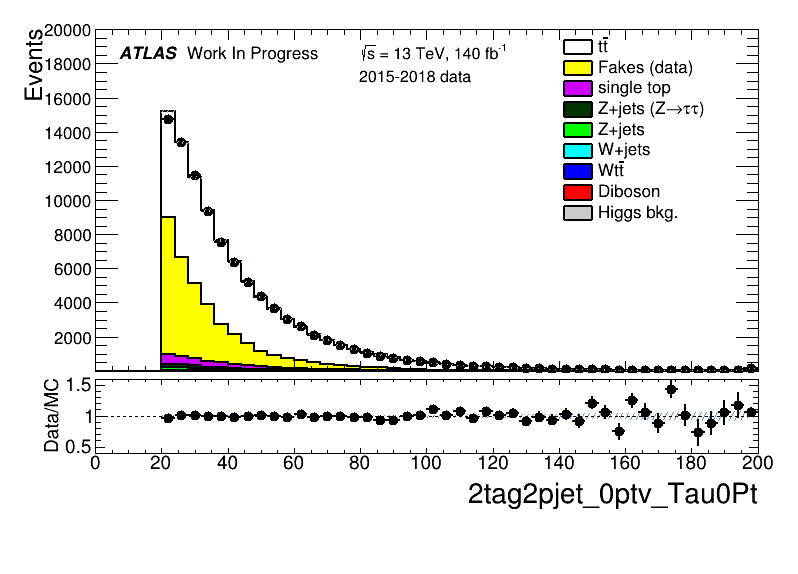
\includegraphics[width=.45\textwidth]{figures/selection/LepHad_HH/2tag2pjet_0ptv_Tau0Pt_SR_ALLFAKES_SLT_ALL_NR_TRBins.png}
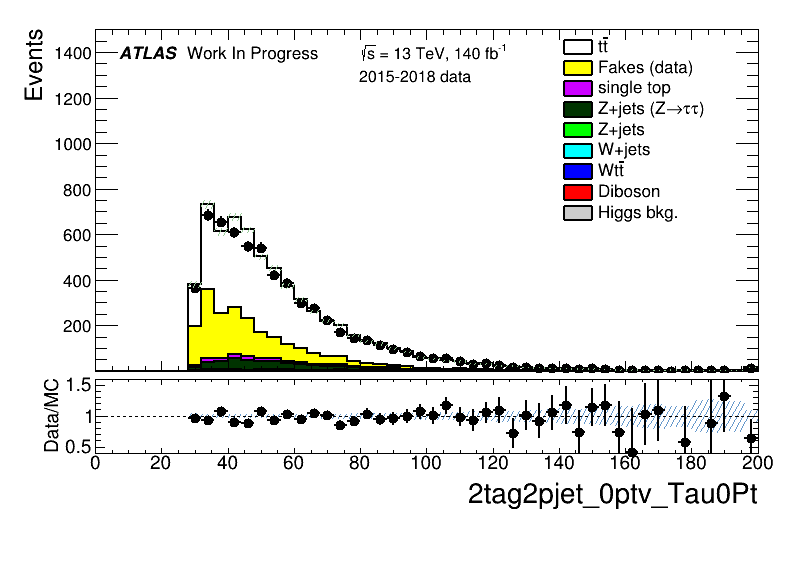
\includegraphics[width=.45\textwidth]{figures/selection/LepHad_HH/2tag2pjet_0ptv_Tau0Pt_SR_ALLFAKES_LTT_ALL_NR_TRBins.png} \\
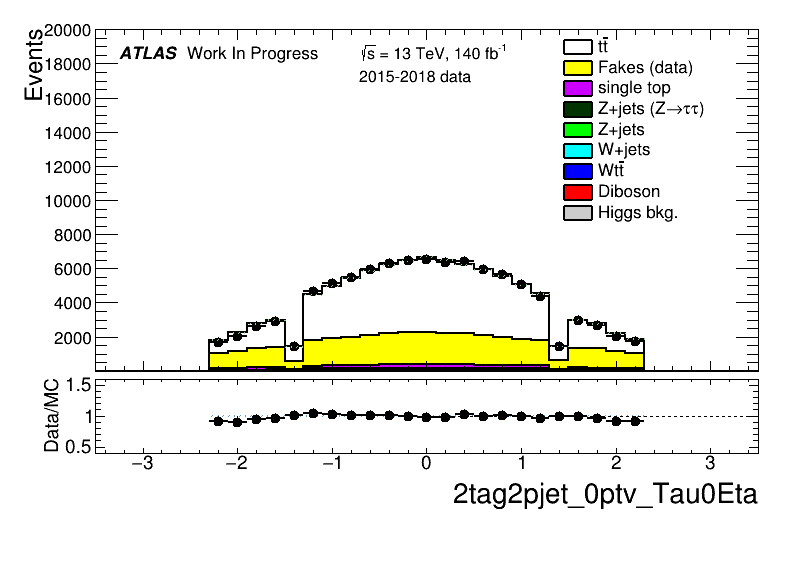
\includegraphics[width=.45\textwidth]{figures/selection/LepHad_HH/2tag2pjet_0ptv_Tau0Eta_SR_ALLFAKES_SLT_ALL_NR_TRBins.png}
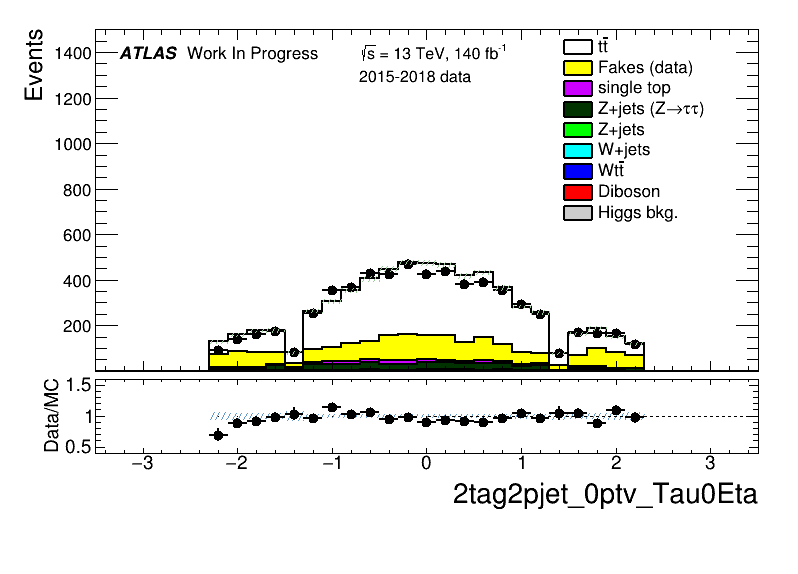
\includegraphics[width=.45\textwidth]{figures/selection/LepHad_HH/2tag2pjet_0ptv_Tau0Eta_SR_ALLFAKES_LTT_ALL_NR_TRBins.png} \\
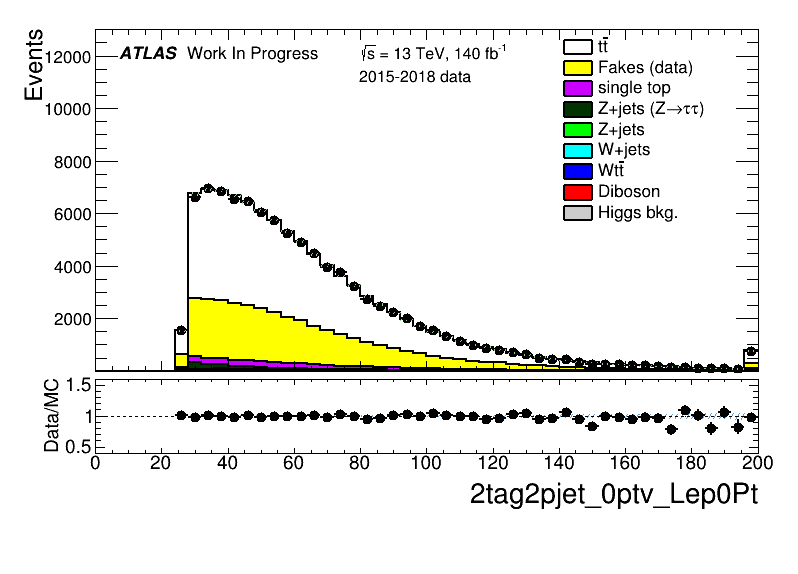
\includegraphics[width=.45\textwidth]{figures/selection/LepHad_HH/2tag2pjet_0ptv_Lep0Pt_SR_ALLFAKES_SLT_ALL_NR_TRBins.png}
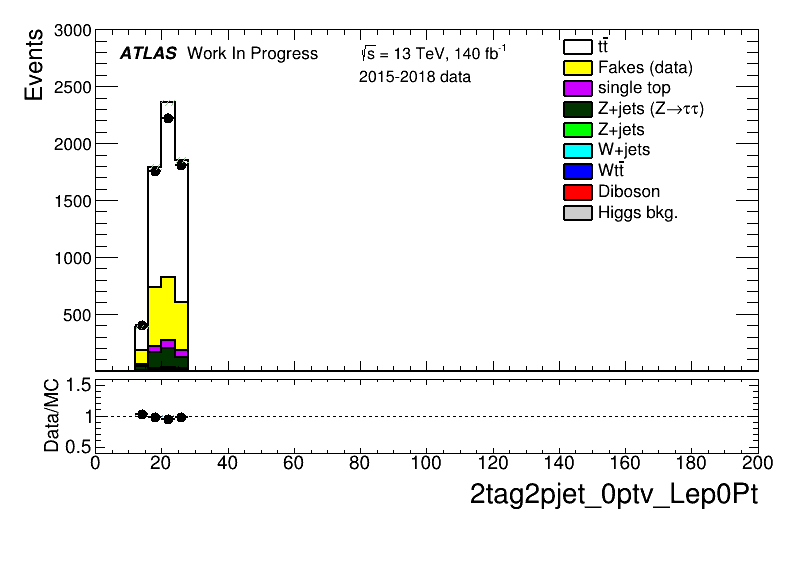
\includegraphics[width=.45\textwidth]{figures/selection/LepHad_HH/2tag2pjet_0ptv_Lep0Pt_SR_ALLFAKES_LTT_ALL_NR_TRBins.png} \\
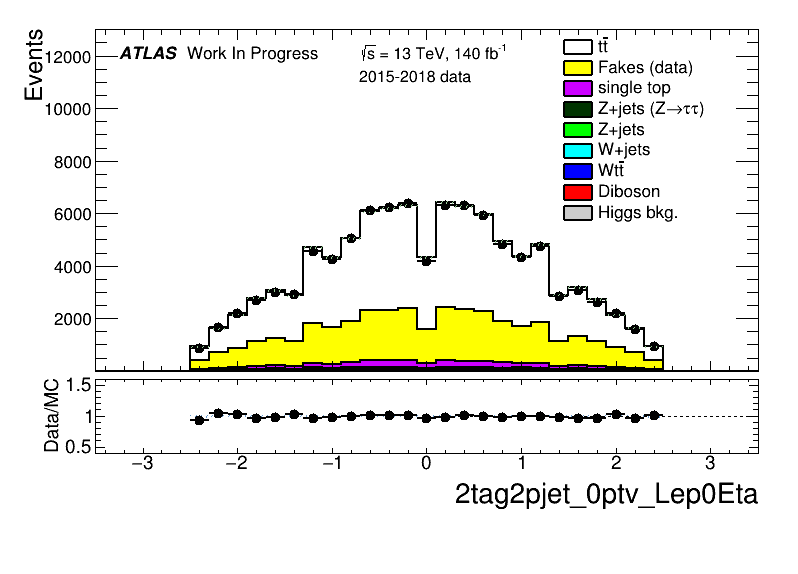
\includegraphics[width=.45\textwidth]{figures/selection/LepHad_HH/2tag2pjet_0ptv_Lep0Eta_SR_ALLFAKES_SLT_ALL_NR_TRBins.png}
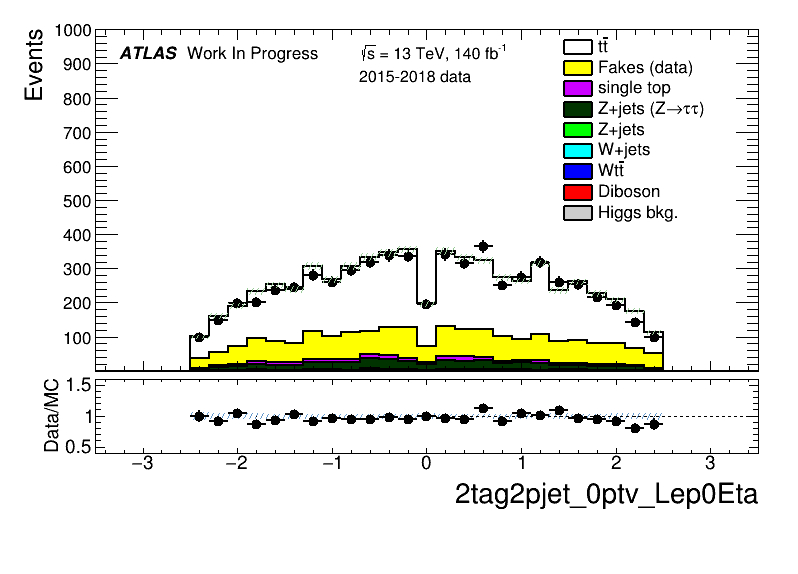
\includegraphics[width=.45\textwidth]{figures/selection/LepHad_HH/2tag2pjet_0ptv_Lep0Eta_SR_ALLFAKES_LTT_ALL_NR_TRBins.png} \\
\caption{Plots of (top row) $\tau$ $p_T$, (second row) $\tau$ $\eta$, (third row) lepton (electron or muon) $p_T$ and (bottom) $\eta$,  for the (left) SLT and (right) LTT trigger channels.}
\label{fig:lh_taulepsel}
\end{figure}


\begin{figure}
\centering
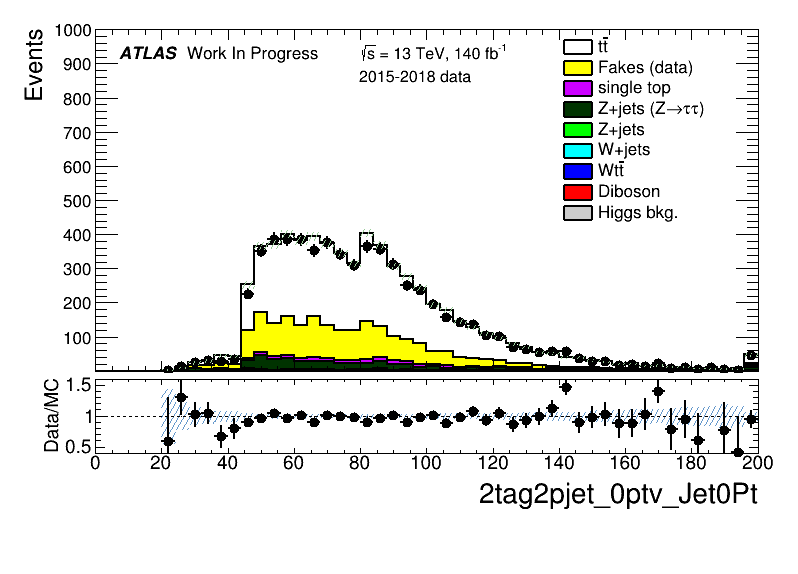
\includegraphics[width=.24\textwidth]{figures/selection/LepHad_HH/2tag2pjet_0ptv_Jet0Pt_SR_ALLFAKES_LTT_ALL_NR_TRBins.png} 
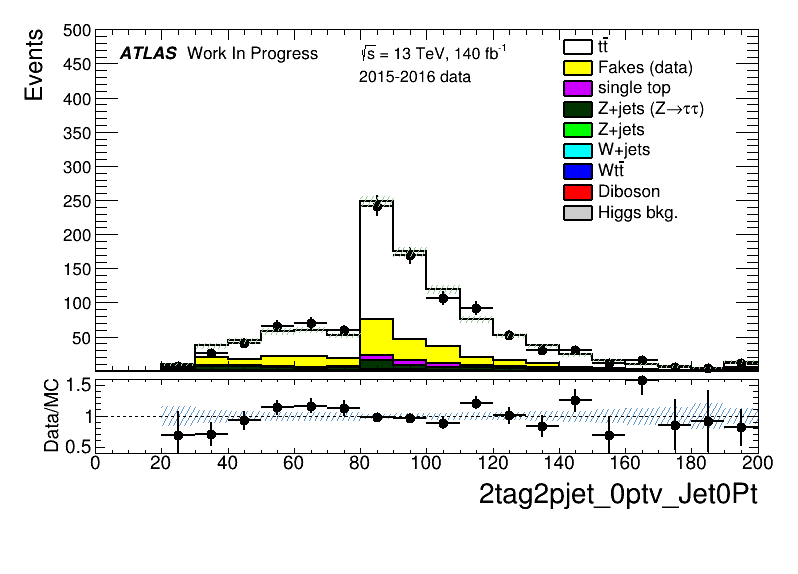
\includegraphics[width=.24\textwidth]{figures/selection/LepHad_HH/2tag2pjet_0ptv_Jet0Pt_SR_ALLFAKES_LTT_2016_TRBins.png} 
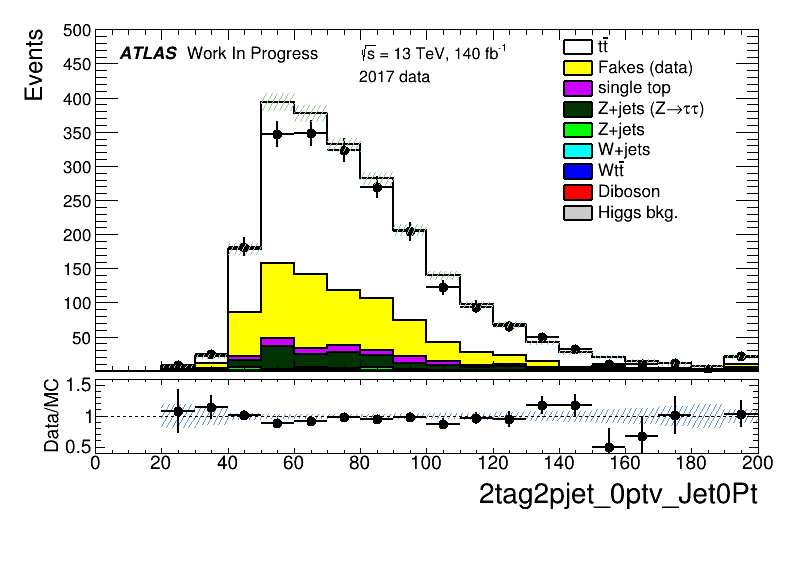
\includegraphics[width=.24\textwidth]{figures/selection/LepHad_HH/2tag2pjet_0ptv_Jet0Pt_SR_ALLFAKES_LTT_2017_TRBins.png} 
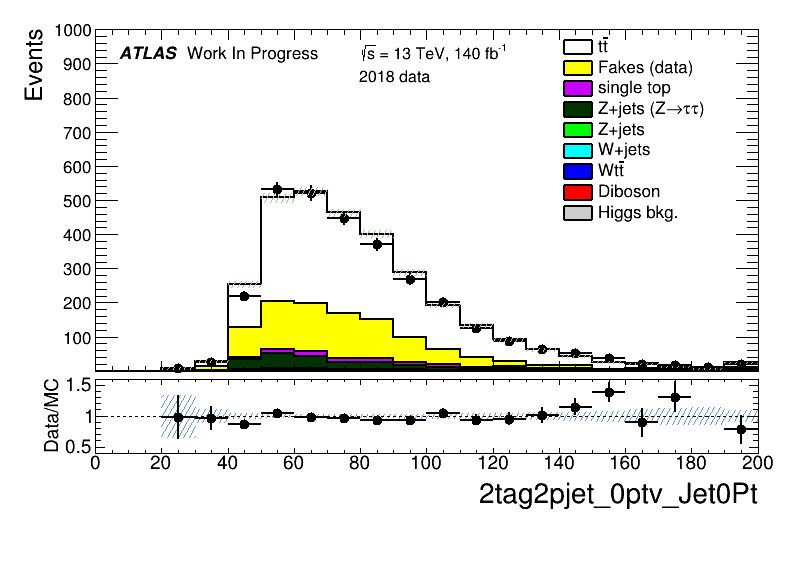
\includegraphics[width=.24\textwidth]{figures/selection/LepHad_HH/2tag2pjet_0ptv_Jet0Pt_SR_ALLFAKES_LTT_2018_TRBins.png} \\
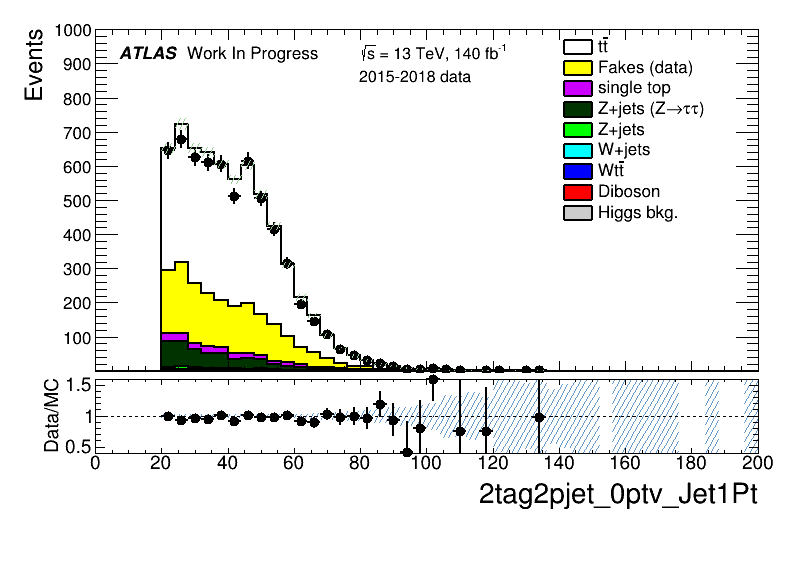
\includegraphics[width=.24\textwidth]{figures/selection/LepHad_HH/2tag2pjet_0ptv_Jet1Pt_SR_ALLFAKES_LTT_ALL_NR_TRBins.png}
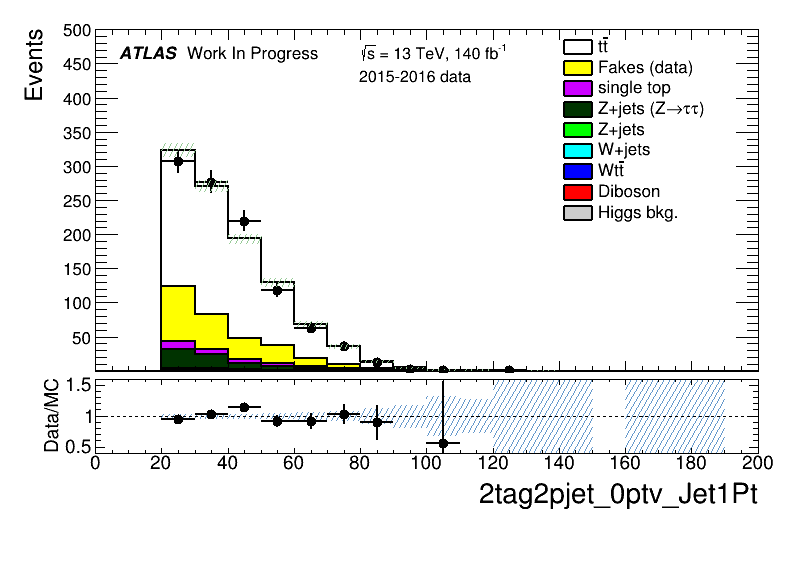
\includegraphics[width=.24\textwidth]{figures/selection/LepHad_HH/2tag2pjet_0ptv_Jet1Pt_SR_ALLFAKES_LTT_2016_TRBins.png}
 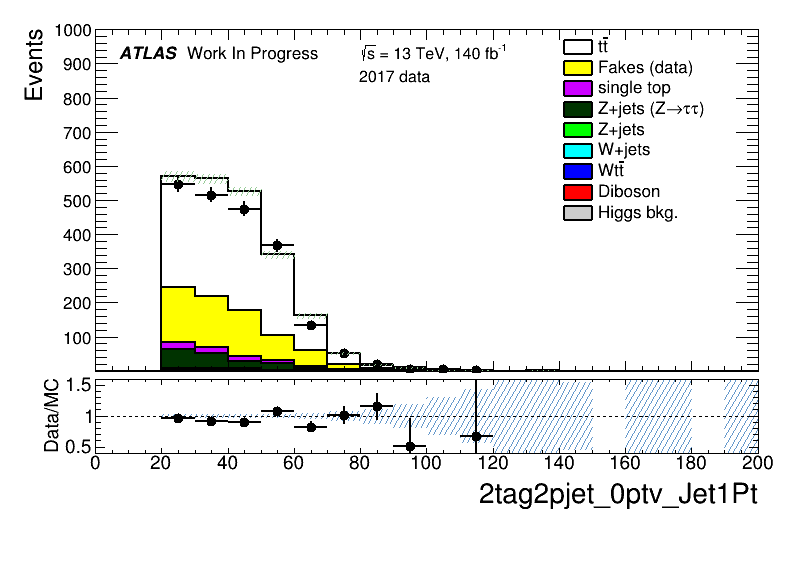
\includegraphics[width=.24\textwidth]{figures/selection/LepHad_HH/2tag2pjet_0ptv_Jet1Pt_SR_ALLFAKES_LTT_2017_TRBins.png}
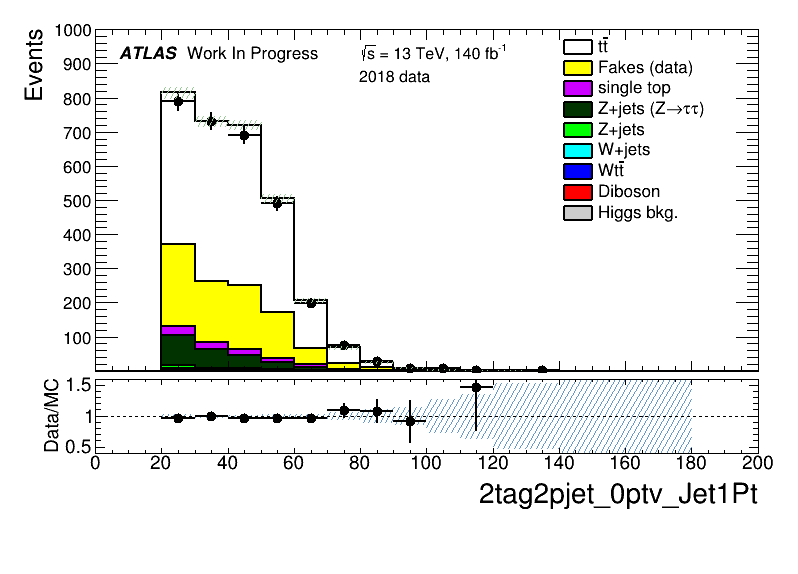
\includegraphics[width=.24\textwidth]{figures/selection/LepHad_HH/2tag2pjet_0ptv_Jet1Pt_SR_ALLFAKES_LTT_2018_TRBins.png} \\
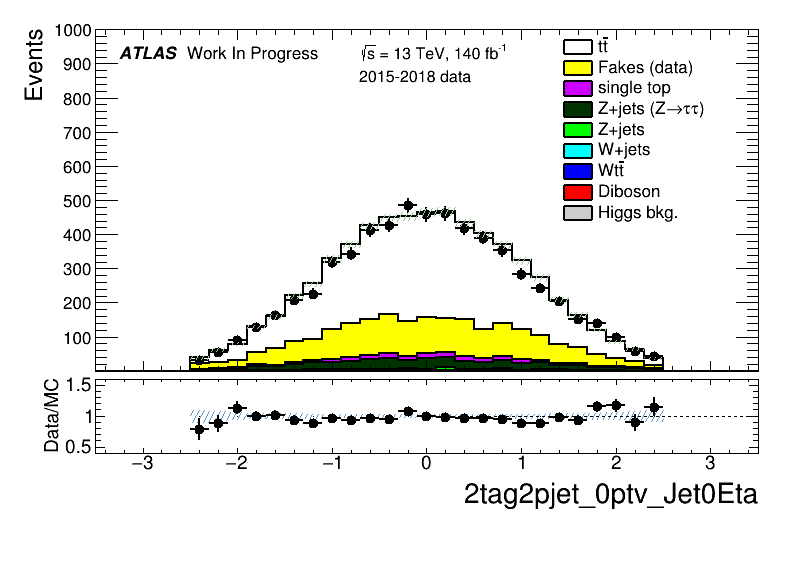
\includegraphics[width=.24\textwidth]{figures/selection/LepHad_HH/2tag2pjet_0ptv_Jet0Eta_SR_ALLFAKES_LTT_ALL_NR_TRBins.png} 
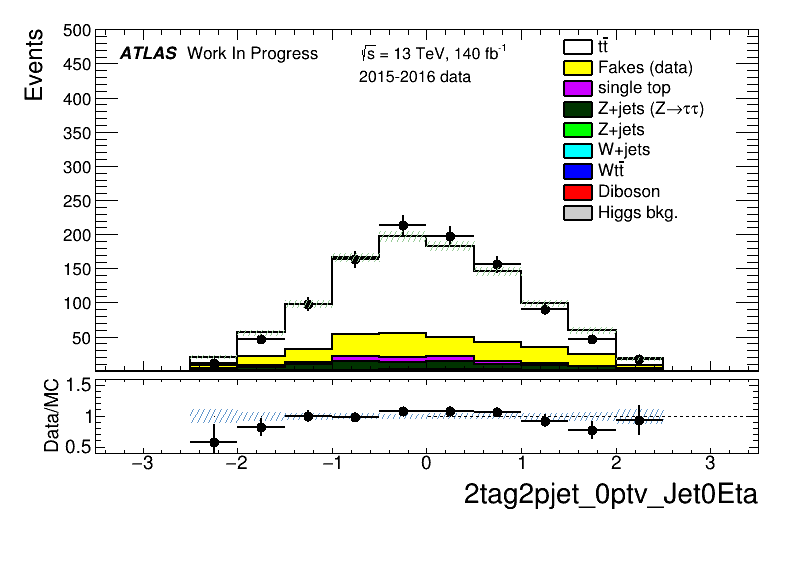
\includegraphics[width=.24\textwidth]{figures/selection/LepHad_HH/2tag2pjet_0ptv_Jet0Eta_SR_ALLFAKES_LTT_2016_TRBins.png} 
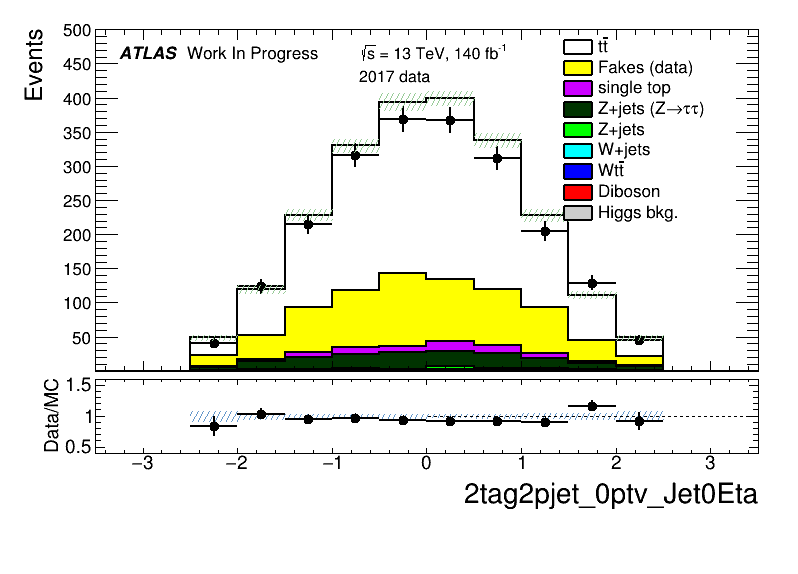
\includegraphics[width=.24\textwidth]{figures/selection/LepHad_HH/2tag2pjet_0ptv_Jet0Eta_SR_ALLFAKES_LTT_2017_TRBins.png} 
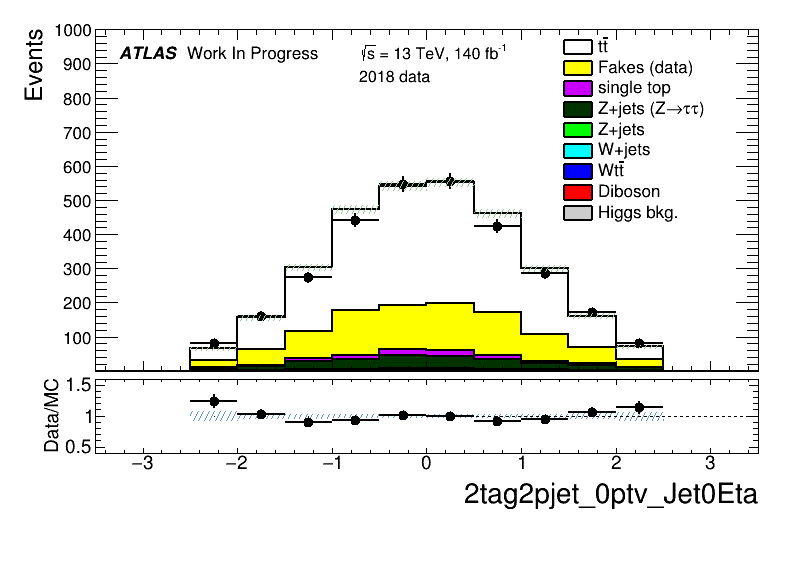
\includegraphics[width=.24\textwidth]{figures/selection/LepHad_HH/2tag2pjet_0ptv_Jet0Eta_SR_ALLFAKES_LTT_2018_TRBins.png} \\
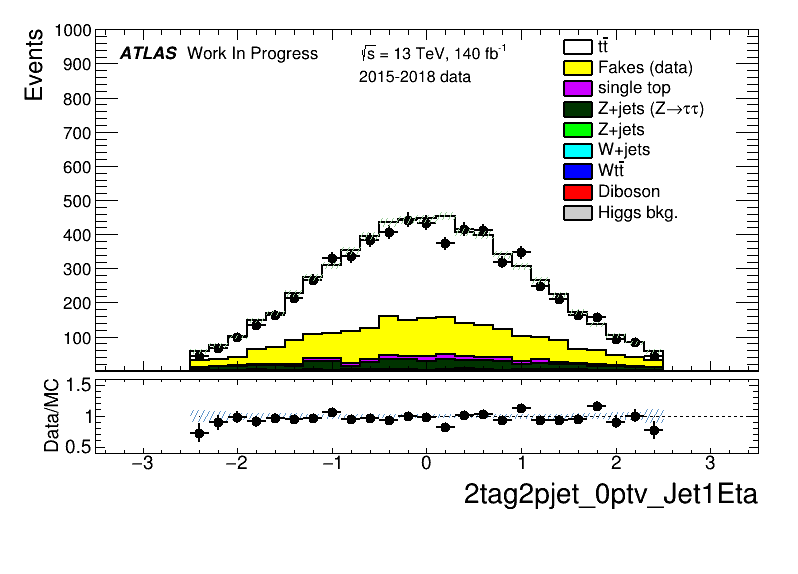
\includegraphics[width=.24\textwidth]{figures/selection/LepHad_HH/2tag2pjet_0ptv_Jet1Eta_SR_ALLFAKES_LTT_ALL_NR_TRBins.png}
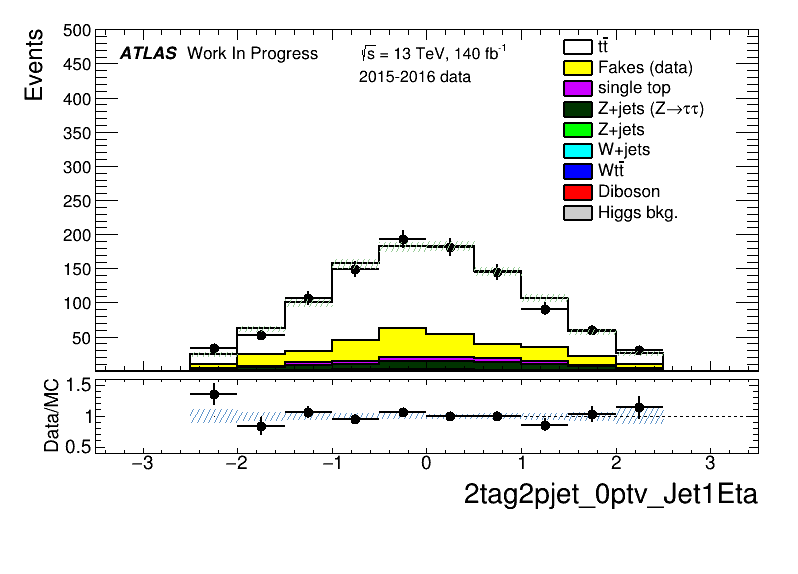
\includegraphics[width=.24\textwidth]{figures/selection/LepHad_HH/2tag2pjet_0ptv_Jet1Eta_SR_ALLFAKES_LTT_2016_TRBins.png}
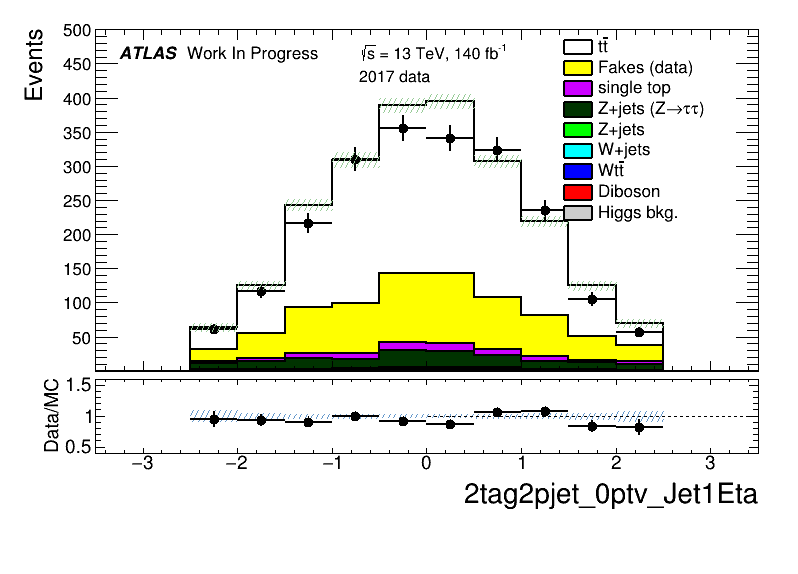
\includegraphics[width=.24\textwidth]{figures/selection/LepHad_HH/2tag2pjet_0ptv_Jet1Eta_SR_ALLFAKES_LTT_2017_TRBins.png}
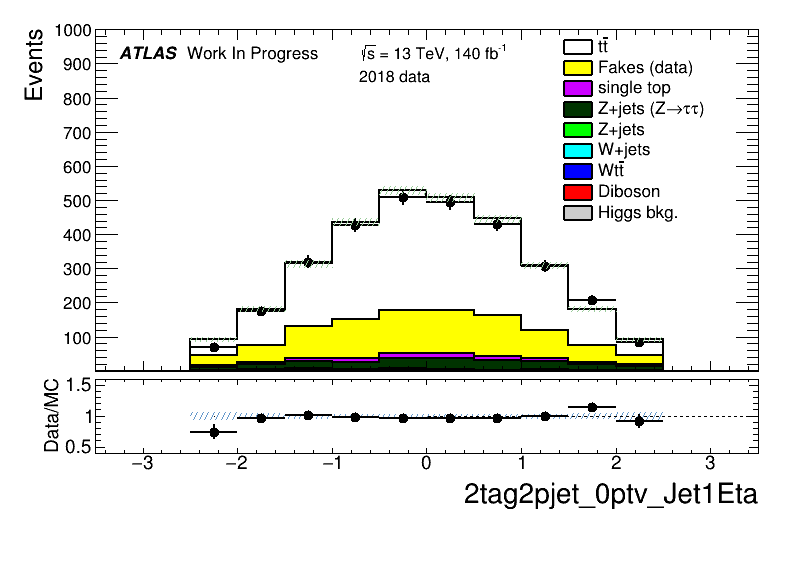
\includegraphics[width=.24\textwidth]{figures/selection/LepHad_HH/2tag2pjet_0ptv_Jet1Eta_SR_ALLFAKES_LTT_2018_TRBins.png}
\caption{Plots of jet $p_T$ and $\eta$ for the LTT trigger channels, specifically the $p_T$ of the (1st row) leading $p_T$ $b$-tagged jet, the (2nd row) second leading $p_T$ $b$-tagged jet, $\eta$ of the (3rd row) leading $p_T$ $b$-tagged jet, and the (4th row) second leading $p_T$ $b$-tagged jet. Shown are the total combined dataset (1st column), the 2015-2016 dataset (2nd column), the 2017 dataset (3rd column) and 2018 dataset (last column). Discontinuities correspond to the offline cuts required by trigger requirements at 80 GeV and 45 GeV for particular data periods.}
\label{fig:lh_jetpteta}
\end{figure}



\FloatBarrier